\documentclass[a4paper]{article}

\usepackage{amssymb,,hyperref,graphicx}

\title{Assignment 3 - Question 4}
\author{Ory Band \texttt{300479425}}
\date{\today}

\newtheorem{thm}{Theorem}

\usepackage{fancyhdr}
\pagestyle{fancy}
\lhead{Ory Band \texttt{300479425}}
\rhead{}
\renewcommand{\headrulewidth}{0.4pt}
\renewcommand{\footrulewidth}{0.4pt}

\begin{document}

\maketitle
\newpage

\section {Question 4}

Perceptron and test code is located at:
\\
\url{https://github.com/oryband/machine-learning/tree/master/ass3}

\subsection {Custom Made Data}

\subsubsection {Seperable Data}

To test my perceptron and LibSVM,
I generated 10,000 samples in $\mathbb{R}^2$, bounded by a 1-radius circle.
The data set was split 7500/2500 for training/testing respectively.

At first I tested the perceptron on a completely seperable data set:
Every sample above a certain threshold (upper diagonal) was marked as positive,
and everything below that as negative.
The perceptron learned very quickly (only 2 iterations), with 100\% success.

\begin{figure}[h!]
    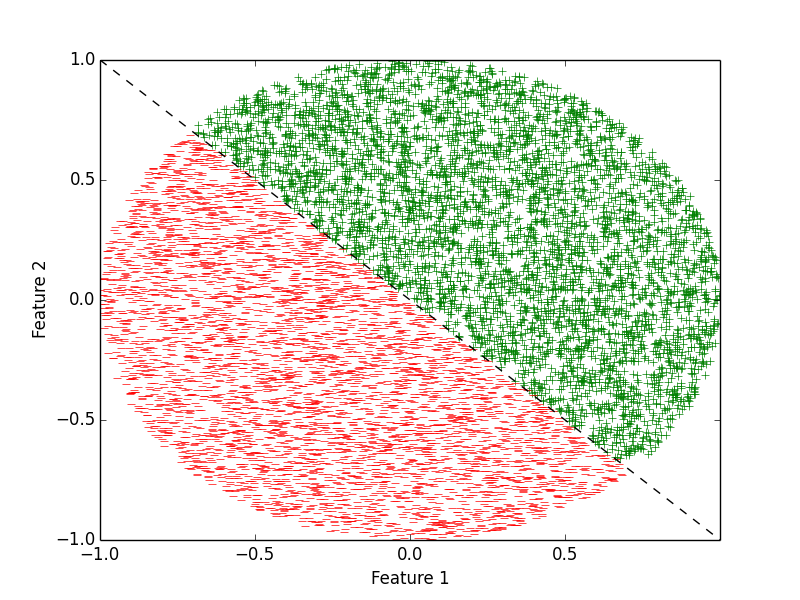
\includegraphics[width=0.5\textwidth]{images/seperable.png}
\end{figure}

LibSVM also didn't have much difficulty learning a how to classify this problem.

\begin{figure}[h!]
    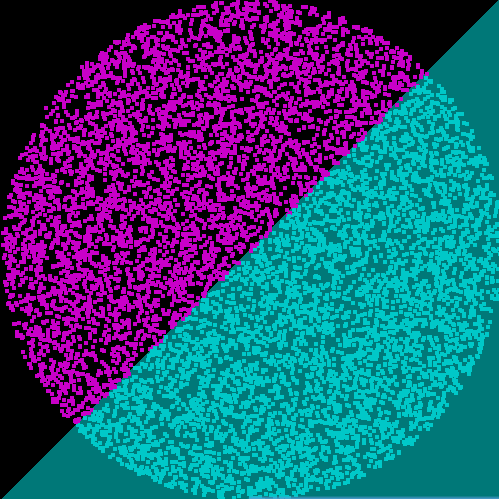
\includegraphics[width=0.5\textwidth]{images/svm_seperable.png}
\end{figure}

\newpage

\subsubsection {Inseperable Data}

Afterwards I regenerated the data set to be inseperable:
I set all samples within a band of 1.4 thickness to be randomly positive
or negative. I tested the success rate as a function of an increasing training
data set, from 1500 to 7500, with a bound of 1000 iterations per size,
and a learning rate of 0.01.
\\\\
All sizes resulted in a 65-70\% success rate, explained by the inseperable data.

\begin{figure}[h!]
    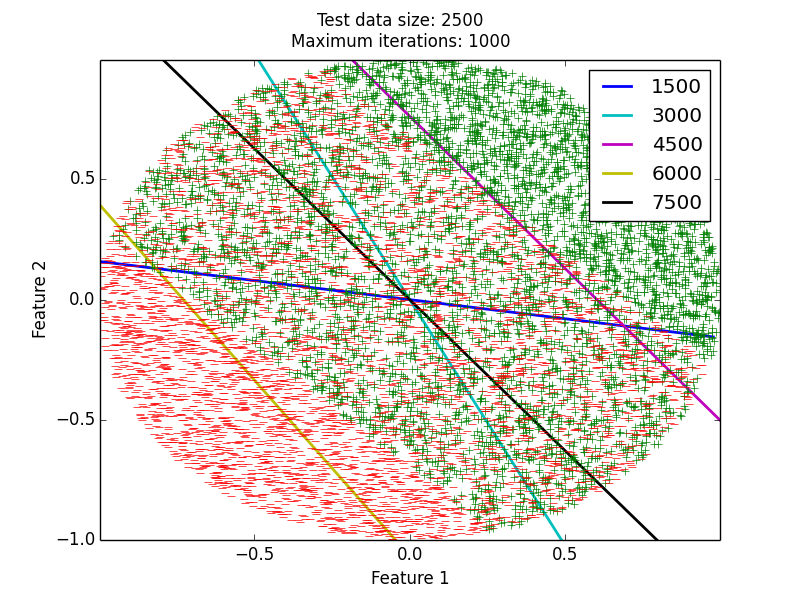
\includegraphics[width=1.0\textwidth]{images/inseperable.png}
    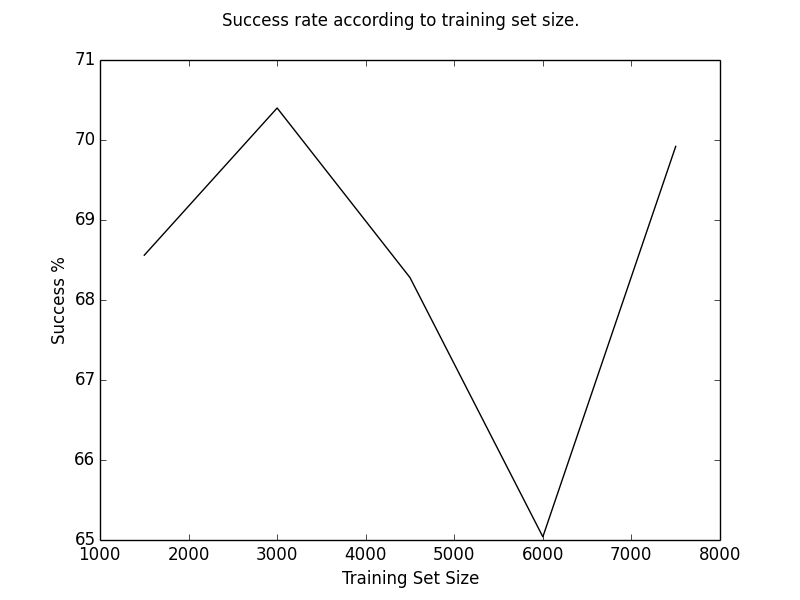
\includegraphics[width=0.8\textwidth]{images/success_rate.png}
\end{figure}

\newpage

I tested SVM with a linear, polynomial, and radial decision kernel functions.
All results were somewhat centered around the center, explained by the fact
that the inseperable data was indeed centered, and the seperable data was at
the edges of the circle. Praticularly, The radial kernel function was very strict
around the edges, and "scrambled" around the center.

\begin{figure}[h!]
    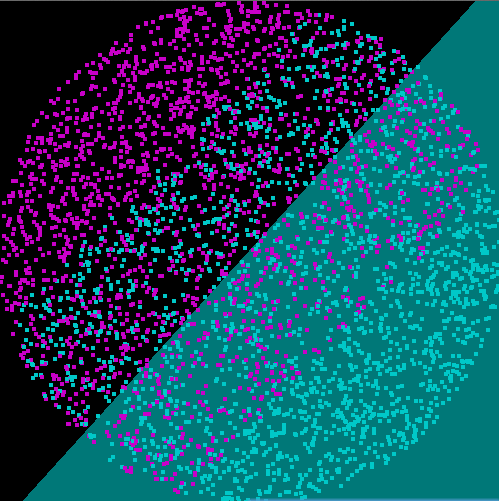
\includegraphics[width=0.5\textwidth]{images/svm_linear.png}
    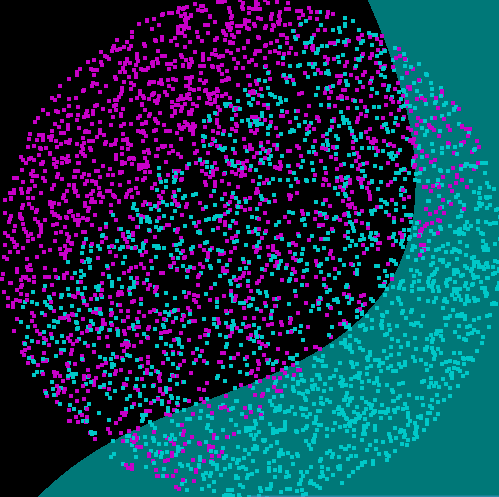
\includegraphics[width=0.5\textwidth]{images/svm_poly.png}
    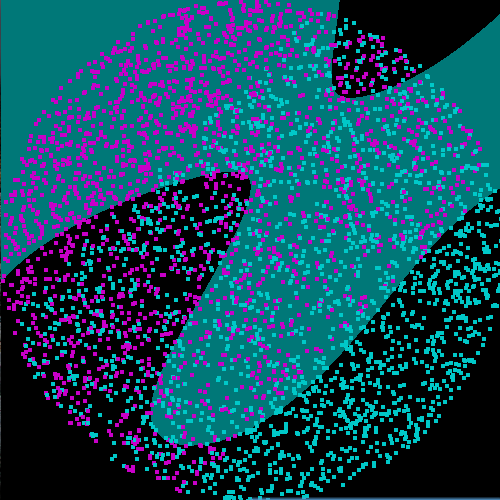
\includegraphics[width=0.5\textwidth]{images/svm_radial.png}
\end{figure}

\newpage

\subsection {Skin Segmentation}

URL: \url{https://archive.ics.uci.edu/ml/datasets/Skin+Segmentation}
\\\\
Afterwards, I tested the perceptron on UCI's skin segmentation data set.
Data was in $\mathbb{R}^3$, and seemed pretty much seperable according to the
results. That is, a very high success rate was achieved, as can be seen in the
graphs on this page.
\\\\
I tested twice with an increasing data set over 10 sizes,
once with a bound of 300 iterations, and then with a bound of 1000.
Both bounds showed a high success rate (about 90\%) on all training sizes.
\\\\
However, I noticed that at every training size,
the perceptron used all the iterations until it reached the iteration bound.
I believe this is due to the data not being completely seperable.
\\\\
Afterwards I tested LibSVM again with linear, polynomial, and radial kernel functions.
Tests concluded with success rate of 93\%, 87\%, and 92\% respectively.
No data-scaling or soft-margins were necessary due to the very high success rate.

\begin{figure}[h!]
    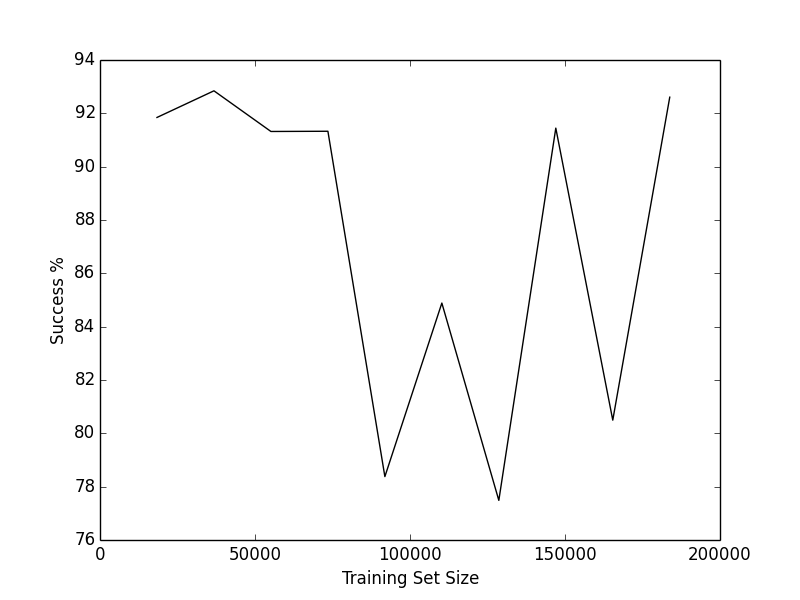
\includegraphics[width=0.5\textwidth]{images/300_iterations.png}
    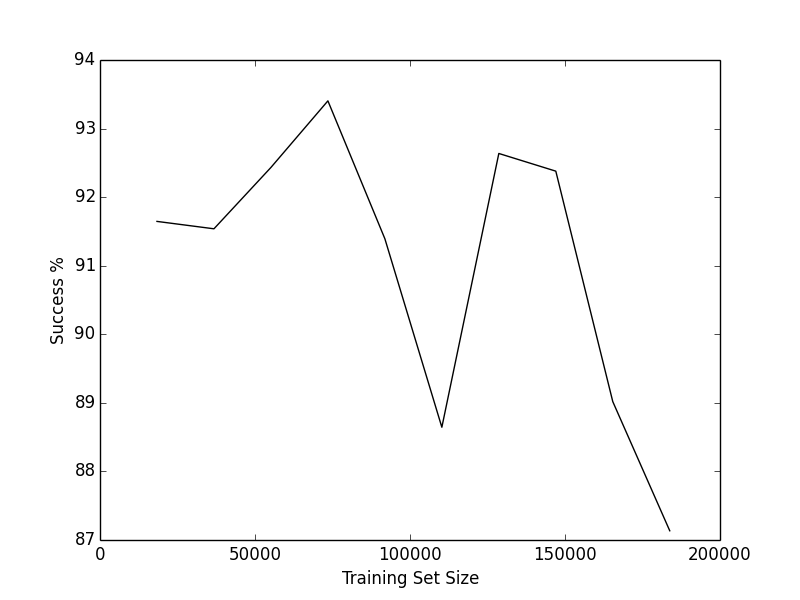
\includegraphics[width=0.5\textwidth]{images/1000_iterations.png}
\end{figure}

\end{document}
